\subsection{Tools}
\begin{itemize}
\item get.py for querying an annotation database
\item what do we have for building an annotation database? (Ann's tool for ingesting the mutrino and jobs info?)
\item framework for working with rdf graph

(plan is to have cataloging and running general queries supported at least, and ideally also slicing-and-fetching of timestamped logs in line-per-timestamp format)
\end{itemize}


- talk about why, eg rdf because it is machine readable, supports adding tools etc over time 


To faciliate the creation of log line annotaitons
and the identification of the occurences of events to be annotated,
we have been using two tools.

LogDiver~\cite{LogDiver} is a tool developed by UIUC which includes a set of regular expressions defining
events in log files of interest; the regular expressions are associated with categorizations
which are a subset of those described in the previous section; the
category name, \texttt{LDxxx}, was chosen to refelct our intention to map to the
Log Diver categroizations where possible.
LogDiver itself is used to discover the occurences of the regular
expresssions in the logs and to determine statistics and infroamtin about event sequences
such as statistics of failure events, or of timigns of failures and recoveries.
LogDiver, or any such regex-based tool (e.g., SEC~\cite{SEC}) can be used to efficiently extract events
and annotate them, based on the intention of the extistence of the regex.

For the dataset descirbed in this work, we prinicpally used Baler~\cite{Baler} for
identifying the log lines to be annotated and for extracing them from the dataset.
Baler extracts patterns from log files without requiring aprior knowledge of
regex. Rather, Baler takes dictionaries of ''words''; words appearing in the log lines
are the passed through to the pattern and non-words become a wildcard in the pattern.
Wildcards of certain formats, for example numbers, hex dumps, char arrays, hostnames and link names
(in cname format for Cray systems) are represented as that formatted type in the pattern.
For example, every instance of the log message \texttt{mutrino-smw 24626 found\_critical\_aries\_error: Processing ''PCI-e CMPL\_TIMEOUT'' critical error (0x660e)}
is represented by the pattern \texttt{<host> nlrd <pid> found\_critical\_aries\_error: Processing ''* *\_TIMEOUT'' critical error (<num>)}.
This illustrates where words, formatted wildcards, and unformatted wildcards (represented by \texttt{*}) appear in the pattern.

For Cray systems, we augment
the dictionary with an architecture specific dictionary of about 100 words (e.g., Lustre, DIMM).
For 3 months of data from our Trinity test system, Mutrino, a 100 node XC 40,
we had over 120 million text log lines which were reduced to 15500 patterns. To further identify patterns
of interest, we weight the patterns by the occurence of 50 weighted
keywords (e.g., congestion = 1.5, error = 1.5, degrade = 0.75). This further reduced the patterns
to 2500 significantly weighted patterns. For example the pattern
\texttt{<host> nlrd <pid> ***ERROR***: Link recovery operation failed; error <num>} has
an aggregate weight of 5.5. From those, we chose 150
patterns to annotate with enhanced descirptions. This resulted in about 860,000
annotated log line instances.

It is our intention to
build a plugin to interface with Baler, and support the annotations there,
however in the prototype, we merely annotated the extracted patterns from
Baler and loaded them into the database.
We do, however, include the Baler pattern id in the annotation fields
for reference ease; only the annotation description, not the original log line nor the pattern
are stored in the annotation database.

Some example patterns, from which the originating log line will be obvious, and
the resulting annotation used in this work, are given in Figure~\ref{f:baler}

\begin{figure*}
\begin{annol}

Baler pattern, preceeded by weight (W=#) and balerpatternid number:
(W=5)        258   HWERR[<host>][<num>]:<num>:SSID RSP A_STATUS_ORB_TIMEOUT Error:*=<num>:*=<num>:*=<num>
Annotation:
authorid:acg  description: 'ORB timeout waiting on outstanding request(s) in the buffer'  LDcatgroup: NE

Baler pattern and weight:
(W=3.75)     498   <host> nlrd <pid> do_set_alerts: <num> links failed, <num> blades failed, <num> blade critical faults, *_in_progress <num>, *_*_reroute <num>; reroute required
Annotation:
authorid:acg  description: 'Setting alerts due to failures. A network reroute is required' LDcatgroup: NE

Baler pattern and weight:
(W=3.25)     748   <host> nlrd <pid> ***ERROR***: Warm swap operation failed; error <num>
Annotation:
authorid:acg description: 'Warm swap failed. This is in response to a operation intended to reset/reinit/replace a component (including network components).' LDcatgroup: NO

Baler pattern and weight:
(W=1.5)      705   <host> nlrd <pid> responder_work_*: Top <num> nodes involved with network congestion
Annotation:
authorid:acg description 'System computing and listing congestion candidate applications' LDcatgroup:NE
\end{annol}
\caption{Example Baler patterns extracted from log lines and their annotated versions. Events to annotate are based on
knowledge of significant events. Annotation descriptions can provide additional context to non-self-explanatory log messages.}
\label{f:baler}
\end{figure*}

\begin{figure*}
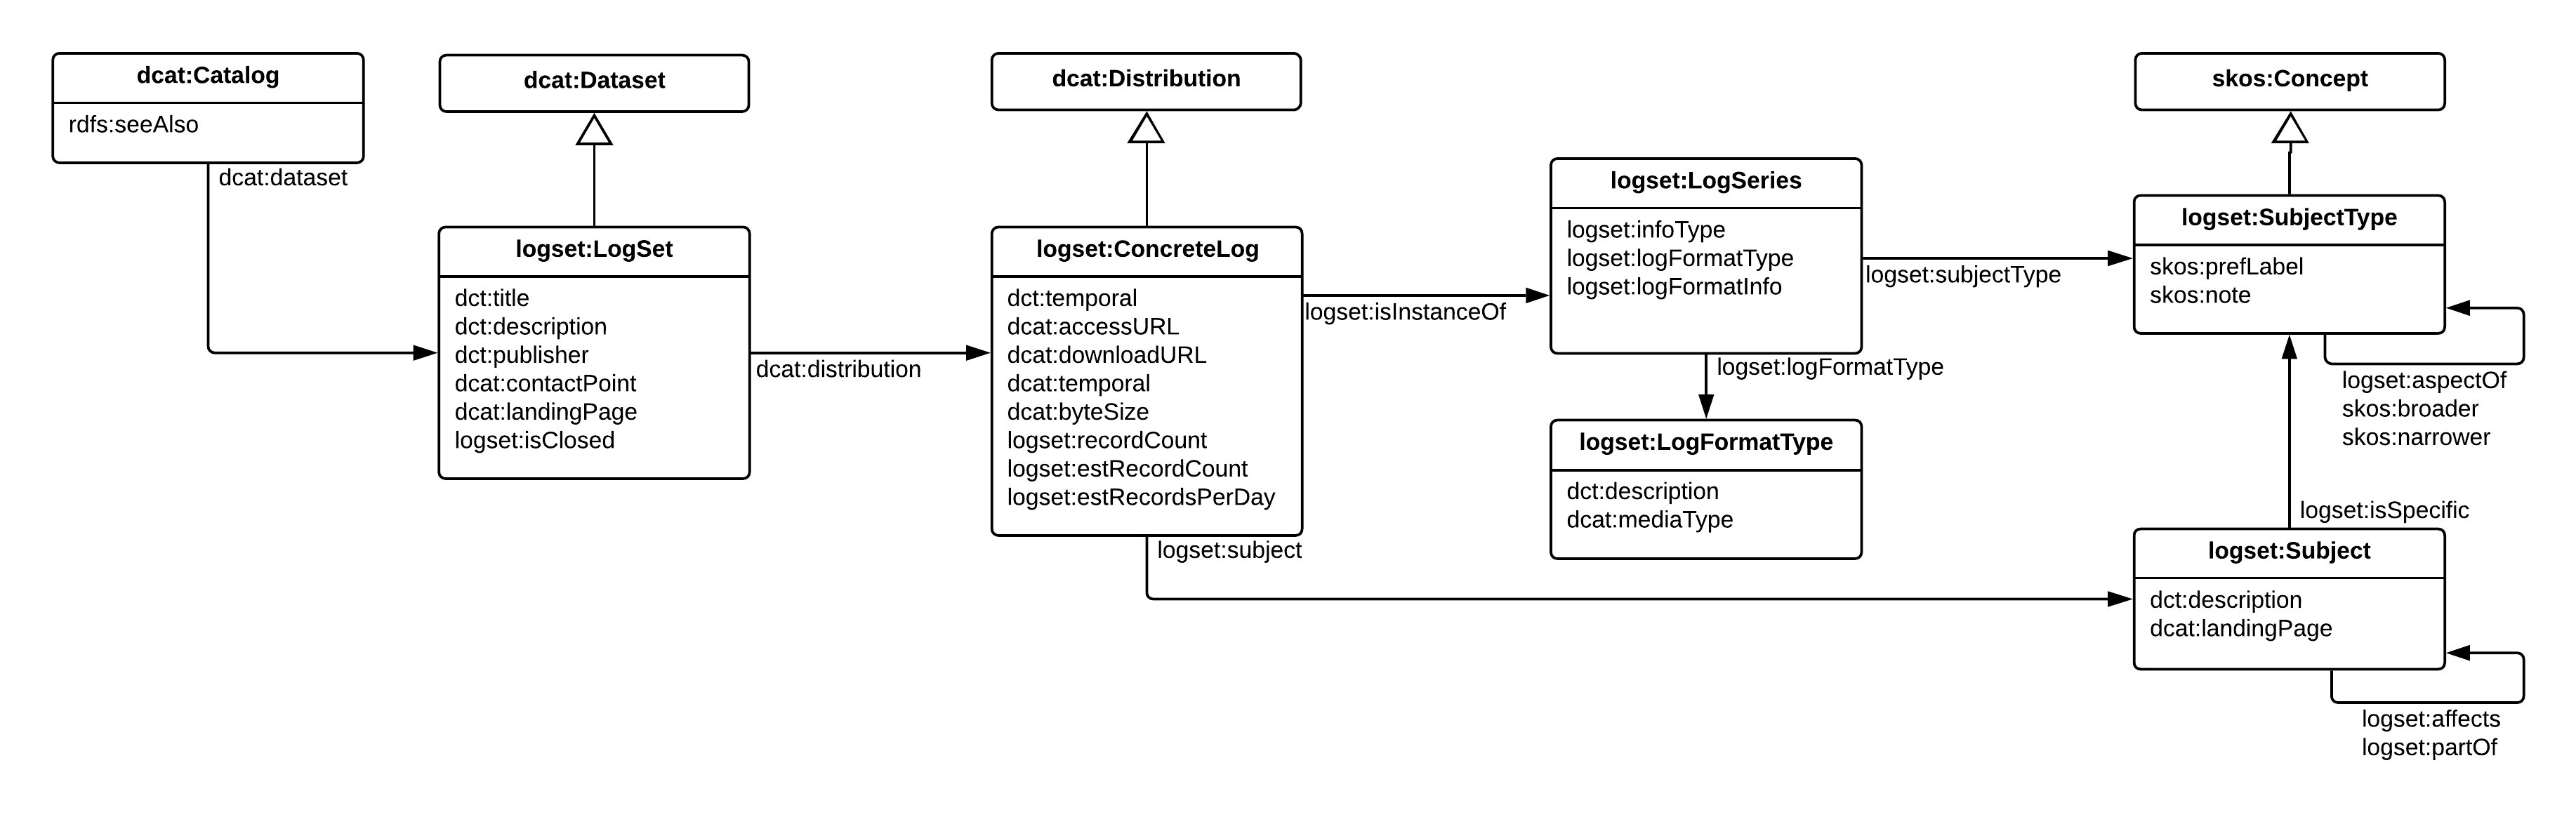
\includegraphics[width=0.9\textwidth]{logset-key-classes.png}
\caption{logset key classes}
\end{figure*}







